\documentclass[conference]{IEEEtran}
\IEEEoverridecommandlockouts
\usepackage{algorithmic}
\usepackage{amsmath,amssymb,amsfonts}
\usepackage{cite}
\usepackage{graphicx}
\usepackage{textcomp}
\usepackage{xcolor}
\def\BibTeX{{\rm B\kern-.05em{\sc i\kern-.025em b}\kern-.08em
    T\kern-.1667em\lower.7ex\hbox{E}\kern-.125emX}}
\begin{document}

\title{
    Fruit Flies:\\
    Developing Flying Orchard Robots
}

\author{
    \IEEEauthorblockN{Michael Hegerhorst}
    \IEEEauthorblockA{michael.hegerhorst@gmail.com}
    \and
    \IEEEauthorblockN{Keaton Anderson}
    \IEEEauthorblockA{keatona379@gmail.com}
    \and
    \IEEEauthorblockN{Caleb Syndergaard}
    \IEEEauthorblockA{caleb.syndergaard@gmail.com}
}

\maketitle

\begin{abstract}
Farmers face numerous challenges when maintaining their crops, one of which is knowing when their crops are ripe.
In particular, orchards can be difficult to manage and fruit can hide in branches.
There is a need to develop a technique to assist farmers in maintaining their orchards.
Modern technologies provide ways to develop models to detect the ripeness of crops, such as apples.
We developed an intelligence hierarchy to use flying drones to assist in the maintenance of orchards by identifying ripe apples.
\end{abstract}


% TODO: Split up by section
% Intro
% Methodology
% Results
% Conclusions
% Etc.
\section{Introduction}
%  Present topic and goal
Farmer's require a lot of land in order to grow their crops. 
In the U.S., apple orchards take up approximately 322 thousand acres of land. %TODO cite acrage of apple orchards line https://www.agmrc.org/commodities-products/fruits/apples
Our project focuses on helping farmer's manage crops across their many acres of land using a drone and machine learning models to 
find apples within the orchard and predict their ripeness and health. By avoiding the need for manual inspection of apples over this large area 
we can lower the time demand for farmer's, and provide a more standardized method of determining crop health by removing the subjectivity of human decision making.\\

%  Existing research
% FIXME: MDH: We don't necessarily need all these sections. Feel free to add or remove as desired.
\section{Background}
\subsection{UAV's in Agriculture}
Although the concept of including Unarmed Aerial Vehicles (UAVs) in agriculture is a rather new concept, there has been some preliminary work done by other researchers on the subject.
Predominately, research conducted in this field has been investigative, rather than relying on actual experimentation.
An example of this is provided in "The influence of drone monitoring on crop health and harvest size", a paper outlining possible uses of drones in the agricultural scene \cite{Reinecke2017}.
During the course of the research conducted by the authors of the aforementioned study, they conducted two interviews. 
The first interview was with UVIRCO, a company "who specialize[s] in cameras and often fit them on drones" and Aerobatics, which is a drone manufacturing company \cite{Reinecke2017}.
The researchers made several conclusions that helped to contribute to our interest in the project.
For examples, they concluded, "drones can be equipped with a multi-spectral camera that can detect the water content underground, which can allow a farmer to determine if a crop row is parched or over-hydrated" \cite{Reinecke2017}.
In addition to this, several other research papers were referenced which concluded 


\section{Methodology}
%  Subsection for each segment of the project?
\begin{figure}[htbp]
    \fontsize{7}{5}\selectfont
    \centering
    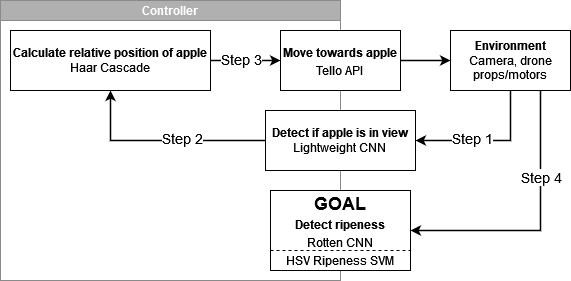
\includegraphics[width=\columnwidth,keepaspectratio]
    {./figures/fruit-fly-model-diagram}
    \caption{
        A data flow diagram of how the intelligence hierarchy works.
        The controller, which operates on another machine receives input from the drone's cameras and other sensors.
        This information is passed to a lightweight model, then to heavier models to operate the drone and determine fruit ripeness.
    }
    \label{fig:fruit-fly-model-diagram}
\end{figure}

\subsection{Initial Object Detection}
I
% TODO cite fruit360
\subsection{Ripeness Detection}
\subsubsection{Data}
The data for this model was a subset of the Fruits 360 data set. % TODO cite
Unable to find any suitable data sets showing a single apple species at different stages of ripeness, we settled for using two ripe, similar looking apple species.
In the Fruits 360 data set, we used crimson snow apples to represent ripe apples, and the data set's "red 2" apples to represent unripe apples. We  chose to use these since the two types had a very similar shape in their images, making the biggest variation between them the color which is what our model focuses on.

\subsubsection{Model}
The ripeness of an apple is determined by an SVM classifier model based on the HSV values of the apple image because it has been shown to be capable of having a high accuracy at fruit ripeness detection\cite{HSVRipeness}.
The model takes an input feature vector based on the histogram calculation of an HSV image, Using OpenCV within python.
Within OpenCV, hue is a number from 0 to 179, inclusive, and saturation and value are both numbers from 0 to 255, inclusive.
The histogram calculation from these results in a 1-dimensional feature vector storing 689 numbers. 
This feature vector is used as input for our SVM classifier.

\subsubsection{Improvements}
Because we were unable to find data focused more specifically on detecting ripeness, the



\input{rotten}




\section{Results}
\autoref{fig:apple-tree-mode-training-curve}
\begin{figure}[!htb]
    \centering
    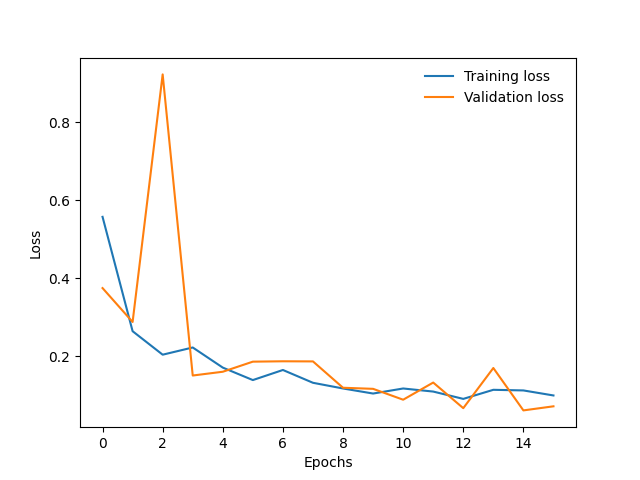
\includegraphics[width=\columnwidth,keepaspectratio]
    {./figures/mobile_model_apple_trees_16its_2022-11-15_training_curve}
    \caption{
        
    }
    \label{fig:apple-tree-mode-training-curve}
\end{figure}


\section{Conclusions}
The goal of our research was to create a drone capable of multi-apple detection and enumeration.
Although we weren't able to create a product capable of accomplishing the initial goal, we were able to provide a ``proof of concept'' model and intelligence hierarchy that, with more time and resources, would provide a way to developing a successful flying drone crop ripeness detector.
The models that we used were consistently lightweight and reportedly capable of performing with minimal training data. 
Although we experienced a decent amount of success using these models, we lacked the data, training time, and compute capacity to create a model that was consistently performant and accurate.
We suspect that given a larger, more diverse dataset, we would be able to produce more accurate models. 
We concluded that despite the shortcomings of a drone, such as short battery life and limited computational power, it was still the best option out of available competing systems.
This is due to the limited nature of its interactions with its environment.
Wheeled systems, specifically skid steer systems, destroy the terrain that they move across. 
The drone is capable of moving throughout the orchard without affecting its surroundings in a physical way.

The code for this project can be found in~\cite{FruitFly}.



\bibliographystyle{IEEEtran}
\begin{small}
    \bibliography{references}
\end{small}

\end{document}
